\addtocontents{toc}{\protect\newpage}
\chapter{Bipartite Clustering} \label{chap:bipartite}

We propose a technique for spectral clustering of bipartite graphs and test its performance on both real and synthetic data.
In Section~\ref{sec:bipartite_graphs} we define bipartite graphs and present our clustering technique.
In Section~\ref{sec:bipartite_sbms} we propose a bipartite stochastic block model (BSBM) and perform experiments with varying parameters.
In Section~\ref{sec:bipartite_american_revolution} we demonstrate our method using the American Revolution network.
In Section~\ref{sec:bipartite_languages} we analyse the Unicode Languages network.






\section{Bipartite graphs} \label{sec:bipartite_graphs}





\begin{definition}
A \emph{bipartite graph} is a graph $\ca{G}=(\ca{V,E})$ where $\ca{V}$ can be partitioned into $\ca{V} = \ca{S} \sqcup \ca{D}$ such that $\ca{E} \subseteq \ca{S} \times \ca{D}$. That is, every edge starts in $\ca{S}$ and ends in $\ca{D}$. We refer to $\ca{S}$ as the \emph{source vertices} and to $\ca{D}$ as the \emph{destination vertices}.
\end{definition}


\subsection{Collider and expander motifs} \label{sec:coll_expa}


Our method for clustering bipartite graphs revolves around two \emph{anchored} motifs; the \emph{collider} and the \emph{expander} (Figure~\ref{fig:expa_coll}). For each motif the anchor set is $\ca{A}=\{ 1,3 \}$.

\begin{figure}[H]
	\centering
	\includegraphics[scale=0.8,draft=false]{../tikz/expa_coll/expa_coll.pdf}
	\caption{The collider and expander motifs}
	\label{fig:expa_coll}
\end{figure}


These motifs are useful for bipartite clustering because of Proposition~\ref{prop:coll_expa_formulae}, which states that their restricted MAMs are the adjacency matrices of the projections~\cite{kolaczyk2014statistical} of the graph $\ca{G}$.
In particular they can be used as similarity matrices for the source and destination vertices respectively.
The similarity of two distinct source (resp. destination) vertices is the sum over their mutual neighbours of the average weights of their edges to (resp. from) that neighbour.

\begin{proposition}[Colliders and expanders in bipartite graphs] \label{prop:coll_expa_formulae}
	Let $\ca{G} = (\ca{V,E},W)$ be a directed bipartite graph. Let $M_\mathrm{coll}$ and $M_\mathrm{expa}$ be the structural or functional MAMs of $\ca{M}_\mathrm{coll}$ and $\ca{M}_\mathrm{expa}$ respectively in $\ca{G}$. Then
%
	\begin{align*}
		(M_\mathrm{coll})_{ij} &= \bb{I} \{i \neq j\} \hspace*{-0.4cm} \sum_{\substack{k \in \ca{D} \\ (i,k), (j,k) \in \ca{E}}} \hspace*{-0.2cm} \frac{1}{2} \Big[ W((i,k)) + W((j,k)) \Big]\,, &(1)\\
		(M_\mathrm{expa})_{ij} &= \bb{I} \{i \neq j\} \hspace*{-0.4cm} \sum_{\substack{k \in \ca{S} \\ (k,i), (k,j) \in \ca{E}}} \hspace*{-0.2cm}\frac{1}{2} \Big[ W((k,i)) + W((k,j)) \Big]\,. &(2)
	\end{align*}
%
\end{proposition}
%
\begin{proof}
See Proof~\ref{proof:coll_expa_formulae}.
\end{proof}




\subsection{Bipartite spectral clustering algorithm}

Algorithm~\ref{alg:bipartite_clustering} gives our procedure for clustering a bipartite graph. The algorithm uses the collider and expander motifs to create similarity matrices for the source and destination vertices respectively (as in Section~\ref{sec:coll_expa}), and then applies random-walk spectral clustering (Algorithm~\ref{alg:rwspectclust}) to produce the partitions.

\vspace*{0.5cm}
\begin{algorithm}[H]
	
	\SetKwFunction{Main}{BipartiteRWSpectClust}				% name of function
	\newcommand{\MainArgs}{$\ca{G},k_\ca{S},k_\ca{D},l_\ca{S},l_\ca{D}$}		% args to function
		
 	\BlankLine
	\Input{Bipartite graph $\ca{G}$, source clusters $k_\ca{S}$, destination clusters $k_\ca{D}$, source dimension $l_\ca{S}$, destination dimension $l_\ca{D}$}
	\Output{Source partition $\ca{S}_1, \ldots, \ca{S}_{k_\ca{S}}$, destination partition $\ca{D}_1, \ldots, \ca{D}_{k_\ca{D}}$}
	\BlankLine
	
	\Function{\Main{\MainArgs}}{
		Construct the collider motif adjacency matrix $M_\mathrm{coll}$ of the graph $\ca{G}$ \\
		Construct the expander motif adjacency matrix $M_\mathrm{expa}$ of the graph $\ca{G}$ \\
		$M_\mathrm{coll} \leftarrow M_\mathrm{coll}[\ca{S,S}]$ \Comm*{restrict rows and columns of $M_\mathrm{coll}$ to $\ca{S}$ \hspace*{0.07cm}}
		$M_\mathrm{expa} \leftarrow M_\mathrm{expa}[\ca{D,D}]$ \Comm*{restrict rows and columns of $M_\mathrm{expa}$ to $\ca{D}$}
		$\ca{S}_1, \ldots, \ca{S}_{k_\ca{S}} \leftarrow$ \texttt{RWSpectClust($M_\mathrm{coll},k_\ca{S},l_\ca{S}$)} \\
		$\ca{D}_1, \ldots, \ca{D}_{k_\ca{D}} \leftarrow$ \texttt{RWSpectClust($M_\mathrm{expa},k_\ca{D},l_\ca{D}$)} \\
	\Return	$\ca{S}_1, \ldots, \ca{S}_{k_\ca{S}}$ and  $\ca{D}_1, \ldots, \ca{D}_{k_\ca{D}}$
	}

	\caption{Bipartite random walk spectral clustering}
	\label{alg:bipartite_clustering}
\end{algorithm}








\section{Bipartite stochastic block models} \label{sec:bipartite_sbms}

We define the \emph{bipartite stochastic block model} (BSBM) \cite{florescu2016spectral} as the DSBM with $k=4$, $n_1 = \dots = n_4=n$ and $F = \begin{psmallmatrix} 0 & 0 & p & q \\ 0 & 0 & q & p \\ 0 & 0 & 0 & 0 \\ 0 & 0 & 0 & 0 \end{psmallmatrix}$ where $p > q$. Figure~\ref{fig:bipartite_bsbm} illustrates the block structure and sparsity matrix of this model. This model partitions the source vertices as $\ca{S} = \ca{S}_1 \sqcup \ca{S}_2$ and the destination vertices as $\ca{D}=\ca{D}_1 \sqcup \ca{D}_2$. Edges exist with high probability from $\ca{S}_1$ to $\ca{D}_1$ and from $\ca{S}_2$ to $\ca{D}_2$.


\begin{figure}[H]
	\centering
	\includegraphics[scale=0.8,draft=false]{../tikz/bipartite_dsbm/bipartite_dsbm.pdf}
	\caption{BSBM block structure and sparsity matrix}
	\label{fig:bipartite_bsbm}
\end{figure}








We test the performance of Algorithm~\ref{alg:bipartite_clustering} with parameters $k_\ca{S} = k_\ca{D} = l_\ca{S} = l_\ca{D} = 2$ on this model.
For comparison we implement the co-clustering method from \cite{dhillon2001co}, which is based on random-walk spectral clustering of the symmetrised adjacency matrix $G+G^\top$.
Figure~\ref{fig:bipartite} shows violin plots over 20 trials of ARI against method, for different sets of parameters $n,p,q$.
Note that if a bipartite graph is connected, then so are $M_\mathrm{coll}$ and $M_\mathrm{expa}$, so we need not consider the largest connected component size $|C|$.
Performance of the two methods is very similar, for source and destination vertices.





\begin{figure}[H]
	\begin{subfigure}{.49\textwidth}
		\centering
		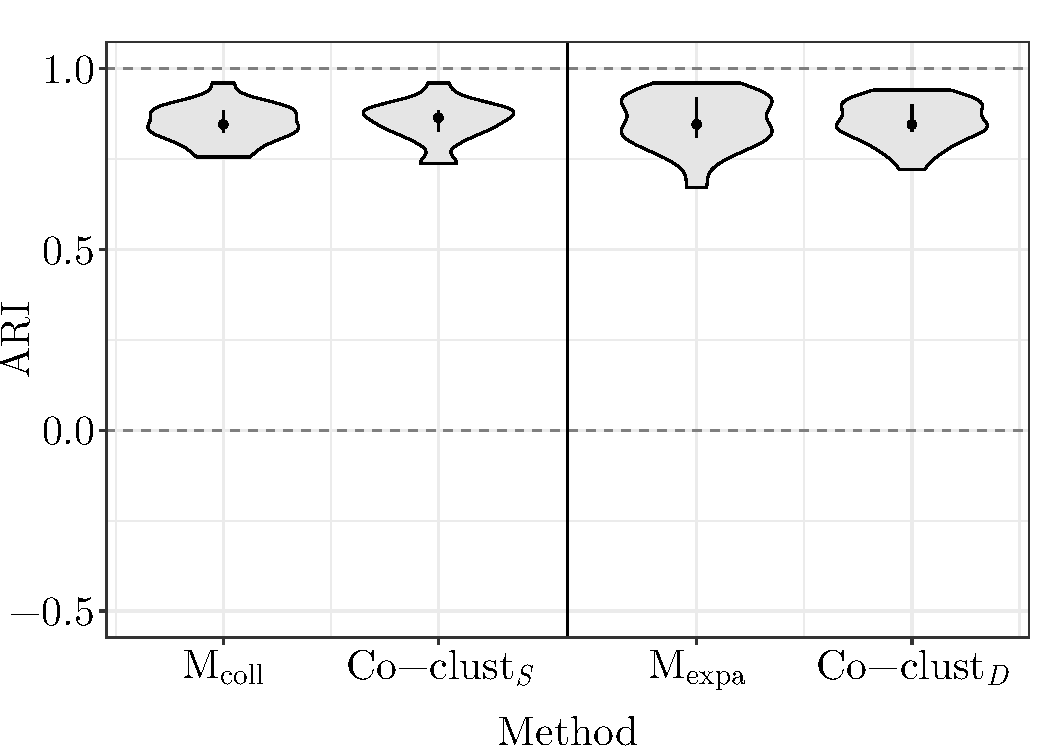
\includegraphics[scale=0.4,draft=false]{../../results/bipartite/bipartite1.pdf}
		\caption{$n=100$, $p=0.2$, $q=0.1$}
	\end{subfigure}
	\begin{subfigure}{.49\textwidth}
		\centering
		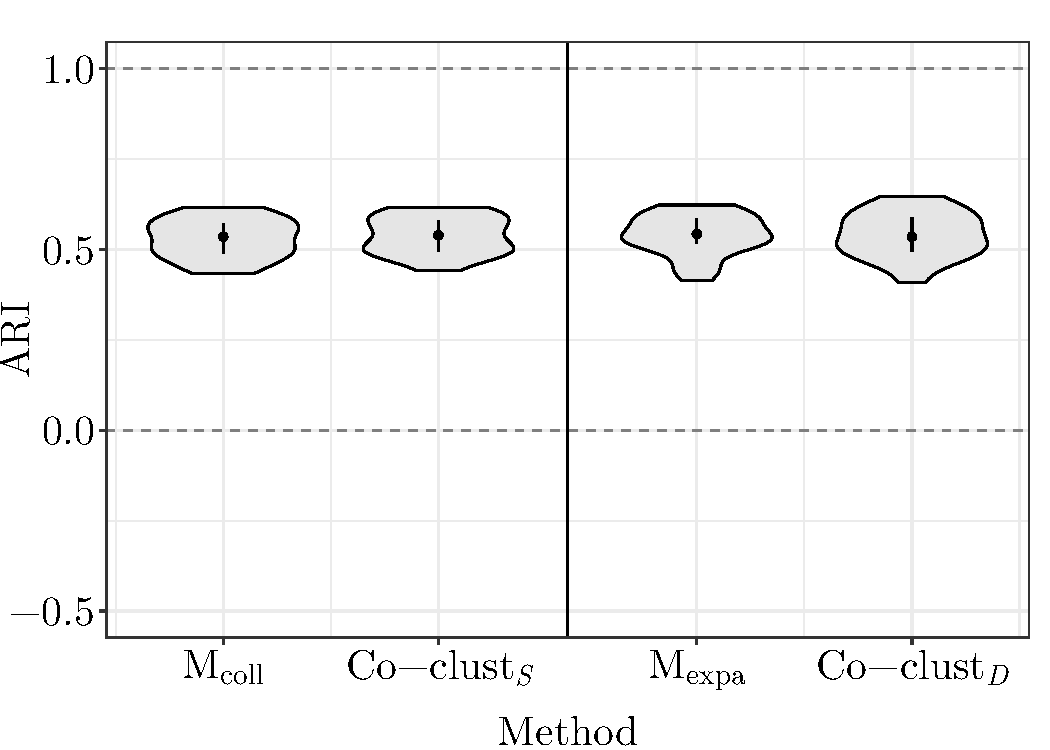
\includegraphics[scale=0.4,draft=false]{../../results/bipartite/bipartite2.pdf}
		\caption{$n=200$, $p=0.1$, $q=0.06$}
	\end{subfigure}
	\caption{ARI violin plots for the BSBM}
	\label{fig:bipartite}
\end{figure}











\section{American Revolution network} \label{sec:bipartite_american_revolution}

As an example of application of our bipartite clustering method to real data, we consider the American Revolution network \cite{konect:brunson_revolution}. This consists of data collected from before the American Revolution. Source vertices are people, and destination vertices are organisations. Edges represent membership of a person to an organisation. There are 136 people, 5 organisations and 160 edges.

Algorithm~\ref{alg:bipartite_clustering} is run on the American Revolution network, with parameters $k_\ca{S} = l_\ca{S} = 5$ and $k_\ca{D} = l_\ca{D} = 2$. Figure~\ref{fig:bipartite_revolution_source} plots the network with people coloured by source cluster, and Figure~\ref{fig:bipartite_revolution_dest} plots the network with organisations coloured by destination cluster. The algorithm succeeds in clustering people based on their common memberships, and in clustering organisations based on their common members.




\begin{figure}[H]
	\begin{subfigure}{.49\textwidth}
		\centering
		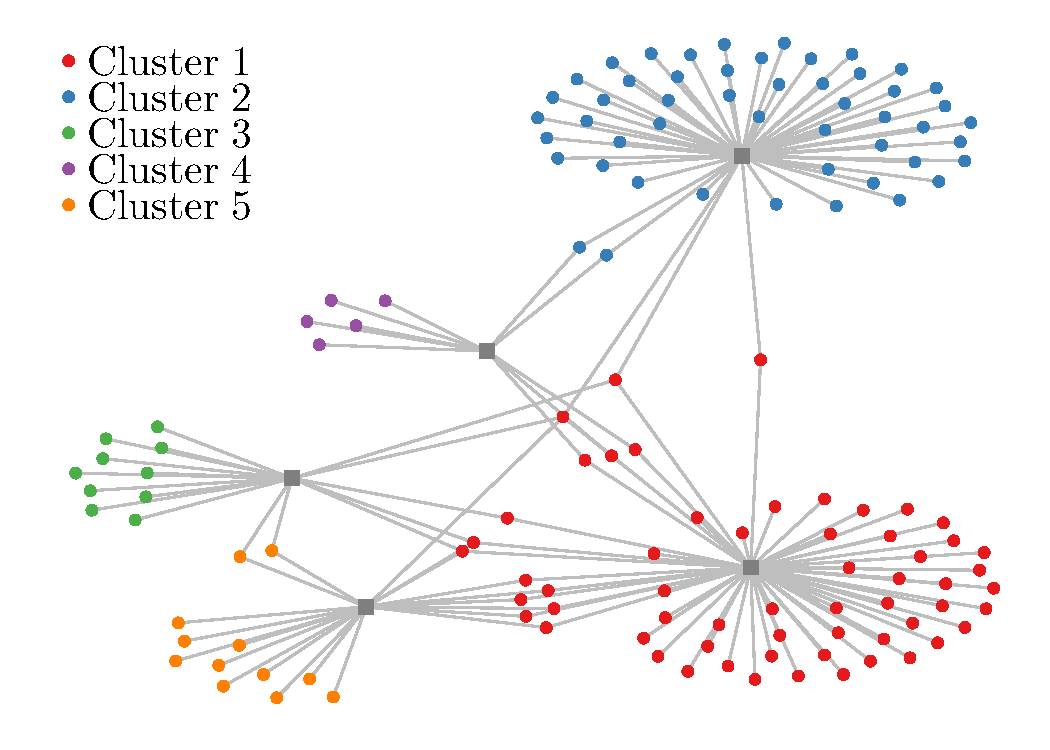
\includegraphics[scale=0.4,draft=false]{../../results/american_revolution/american_revolution_source.pdf}
		\caption{Grouping people into 5 clusters}
		\label{fig:bipartite_revolution_source}
	\end{subfigure}
	\begin{subfigure}{.49\textwidth}
		\centering
		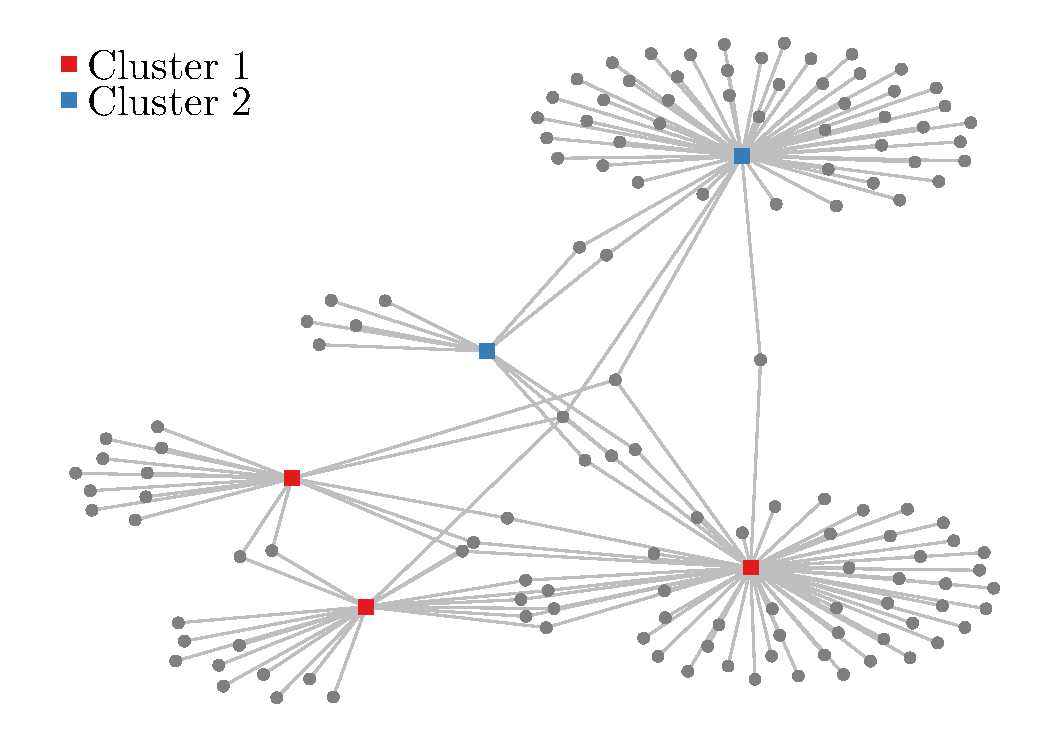
\includegraphics[scale=0.4,draft=false]{../../results/american_revolution/american_revolution_dest.pdf}
		\caption{Grouping organisations into 2 clusters}
		\label{fig:bipartite_revolution_dest}
	\end{subfigure}
	\caption{Bipartite clustering of the American Revolution network}
	\label{fig:bipartite_revolution}
\end{figure}














\section{Unicode Languages network} \label{sec:bipartite_languages}

The final data set is the Unicode Languages network \cite{konect:unicodelang}, consisting of data collected in 2014 on languages spoken around the world.
Source vertices are territories, and destination vertices are languages.
Weighted directed edges from territory to language indicate the number of inhabitants in that territory who speak the specified language (territory population data taken from \cite{geonames}).
After preprocessing (Section~\ref{sec:notes_preprocessing}) there are $155$ territories, $270$ languages and $705$ edges.

We test Algorithm~\ref{alg:bipartite_clustering} with parameters $k_\ca{S} = l_\ca{S} = k_\ca{D} = l_\ca{D} = 6$ on this network.
For the source vertices, Figure~\ref{fig:bipartite_languages_map} plots maps of the world with territories coloured by the clustering obtained. The top 20 territories (by population) in each cluster are given in Table~\ref{tab:bipartite_languages_source_clusters}. 
Cluster~1 is by far the largest cluster, and includes a wide variety of territories, of which many but not all speak some English.
Cluster~2 contains the Persian-speaking territories of Iran and Afghanistan, the Arabic territories of Saudi Arabia and Syria, and the African French-speaking DR Congo, C\^ote d'Ivoire, Burkina Faso, Niger and others. It also includes Haiti, another French-speaking territory.
Cluster~3 mostly captures Spanish-speaking territories in the Americas and also contains Equatorial Guinea, another Spanish-speaking territory in Africa.
Cluster~4 includes the Slavic territories of Russia and some of its neighbours. The absence of Kazakhstan may be due to the $981 \, 760$ Kazakhs who speak German which is not a Slavic or Turkic language.
Cluster~5 covers China, Hong Kong, Mongolia and some of South-East Asia. The inclusion of Panama might be due to the $6821$ Panamanians who speak Chinese.
Cluster~6 is the smallest cluster and contains only Japan and the Koreas, which are connected by the $636 \, 440$ Japanese who speak Korean.

There are a few territories and languages which are not contained in the large connected component of the network due to their linguistic isolation. These territories are Laos, Norway and Timor-Leste, and the languages are Lao, Norwegian Bokm{\aa}l and Norwegian Nynorsk.



\begin{figure}[H]
	\centering
	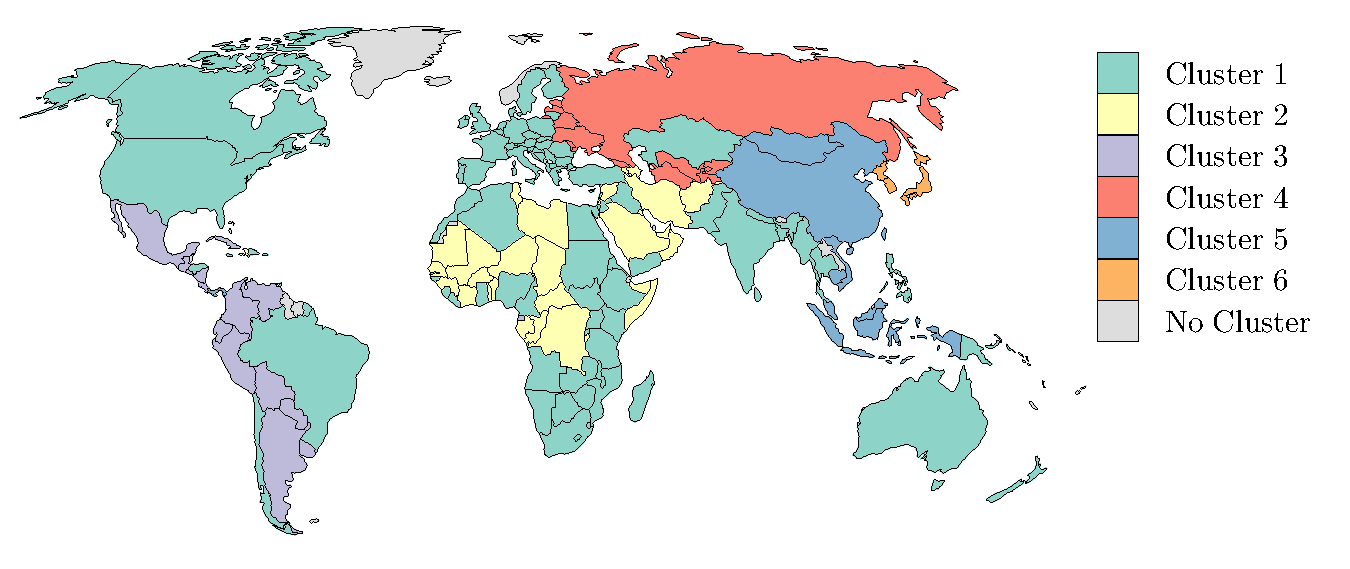
\includegraphics[scale=0.6, draft=false]{../../results/languages/languages_source_map_clusts.pdf}
	\caption{Clustering the territories from the Unicode Languages network}
	\label{fig:bipartite_languages_map}
\end{figure}




\begin{table}[H]
\centering
\scriptsize
	\begin{tabular}{ |c|c|c|c|c|c| }
		\hline	
		\rule{0pt}{1.2em}
		\input{../../results/languages/languages_source_clusters.txt} \\[0.1cm]	
		\hline	
	\end{tabular}
	\caption{Clustering the territories from the Unicode Languages network}
	\label{tab:bipartite_languages_source_clusters}
\end{table}






For the destination vertices, we present the six clusters obtained by Algorithm~\ref{alg:bipartite_clustering}.
Table~\ref{tab:bipartite_languages_dest_clusters} contains the top 20 languages (by number of speakers) in each cluster.
Cluster~1 is the largest cluster and contains the European languages of Spanish, Portuguese and French, as well as dialects of Arabic. 
Cluster~2 is also large and includes English as well as several South Asian languages such as Hindi, Bengali, Urdu and Punjabi.
Cluster~3 consists of many indigenous African languages such as Swahili, Kinyarwanda and Somali.
Cluster~4 captures languages from South-East Asia, mostly spoken in Indonesia and Malaysia.
Cluster~5 identifies several varieties of Chinese and a few other Central and East Asian languages such as Kazakh and Uighur. Interestingly Korean is also placed in this group and not with Japanese, even though the Koreas are clustered together with Japan in Table~\ref{tab:bipartite_languages_source_clusters}.
Cluster~6 captures more South-East Asian languages, this time from Thailand, Myanmar and Cambodia. Pattani Malay is in this cluster because despite its name it is spoken more in Thailand than in Malaysia.



\vspace*{0.5cm}
\begin{table}[H]
\centering
\scriptsize
	\begin{tabular}{ |c|c|c|c|c|c| }
		\hline	
		\rule{0pt}{1.2em}
		\input{../../results/languages/languages_dest_clusters.txt} \\[0.1cm]	
		\hline	
	\end{tabular}
	\caption{Clustering the languages from the Unicode Languages network}
	\label{tab:bipartite_languages_dest_clusters}
\end{table}



